\documentclass{article}

% Language setting
% Replace `english' with e.g. `spanish' to change the document language
\usepackage[english]{babel}

% Set page size and margins
% Replace `letterpaper' with `a4paper' for UK/EU standard size
\usepackage[a4paper,top=2cm,bottom=2cm,left=3cm,right=3cm,marginparwidth=1.75cm]{geometry}

% Useful packages
\usepackage{amsmath}
\usepackage{graphicx}
\usepackage[colorlinks=true, allcolors=blue]{hyperref}

\title{TDT4171 — Artificial Intelligence Methods \\ Assignment 9 - Reinforcement Learning}
\author{Erik Storås Sommer - 535006}
\date{March 2023}

\begin{document}
\maketitle
\setlength{\parindent}{0pt}

\section*{Value Iteration}

The value iteration algorithm finds the optimal policy for a given MDP.
The results are shown in the following sections.

\subsection*{Utilities}

The utilities for the states are shown in Figure \ref{fig:image1}.

\begin{figure}[hbtp]
    \centering
    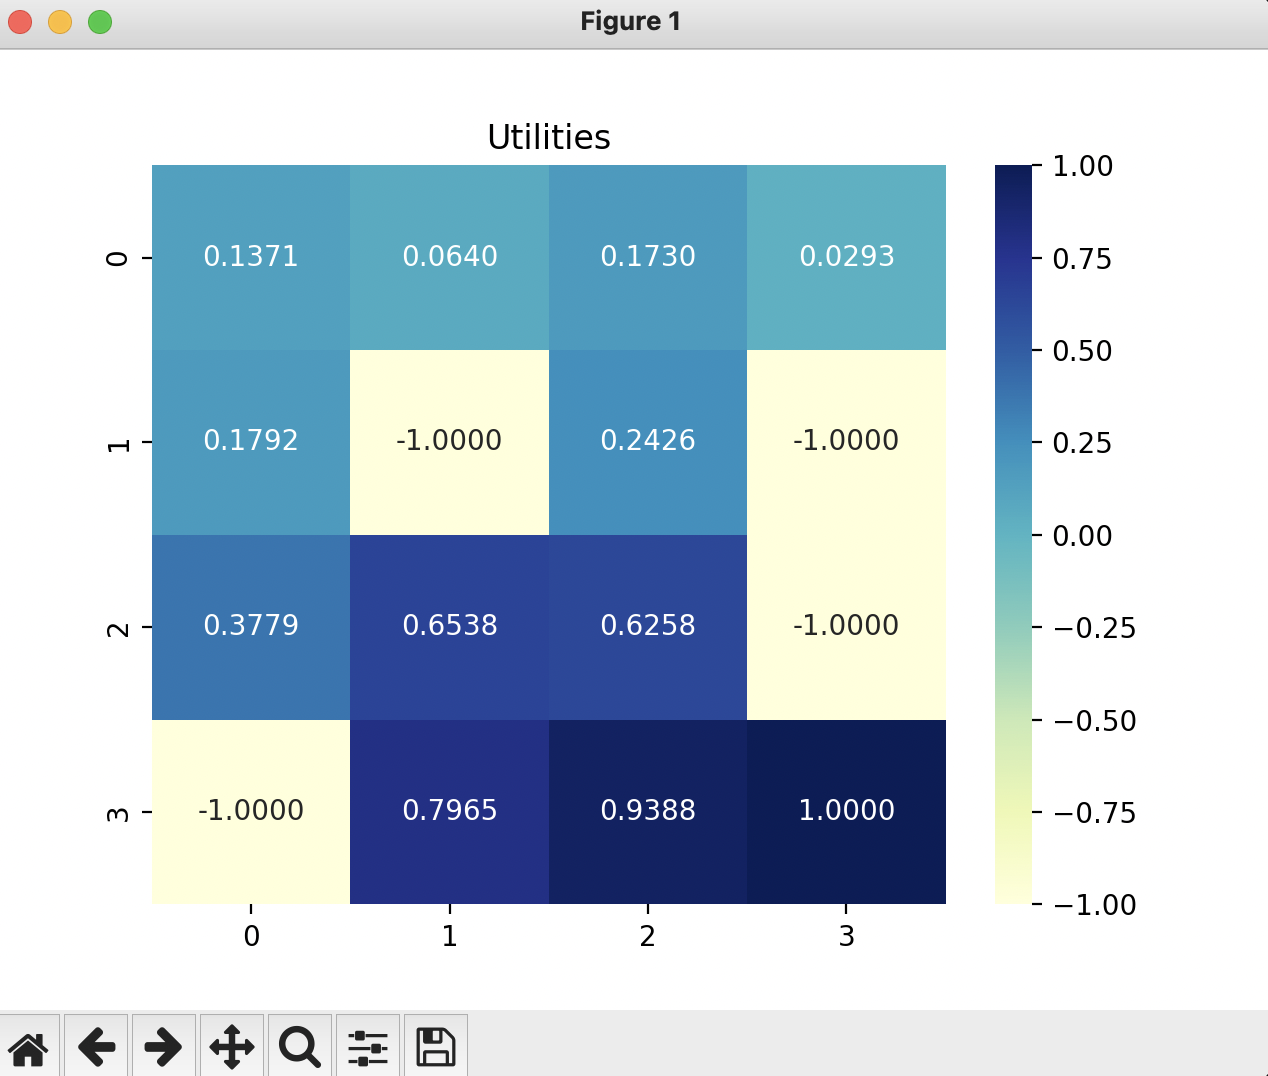
\includegraphics[width=0.85\textwidth]{images/utilities.png}
    \caption{Utilities for the states}
    \label{fig:image1}
\end{figure}

\newpage

\subsection*{Greedy Policy}

The greedy policy for the states are shown in Figure \ref{fig:image2}.

\begin{figure}[hbtp]
    \centering
    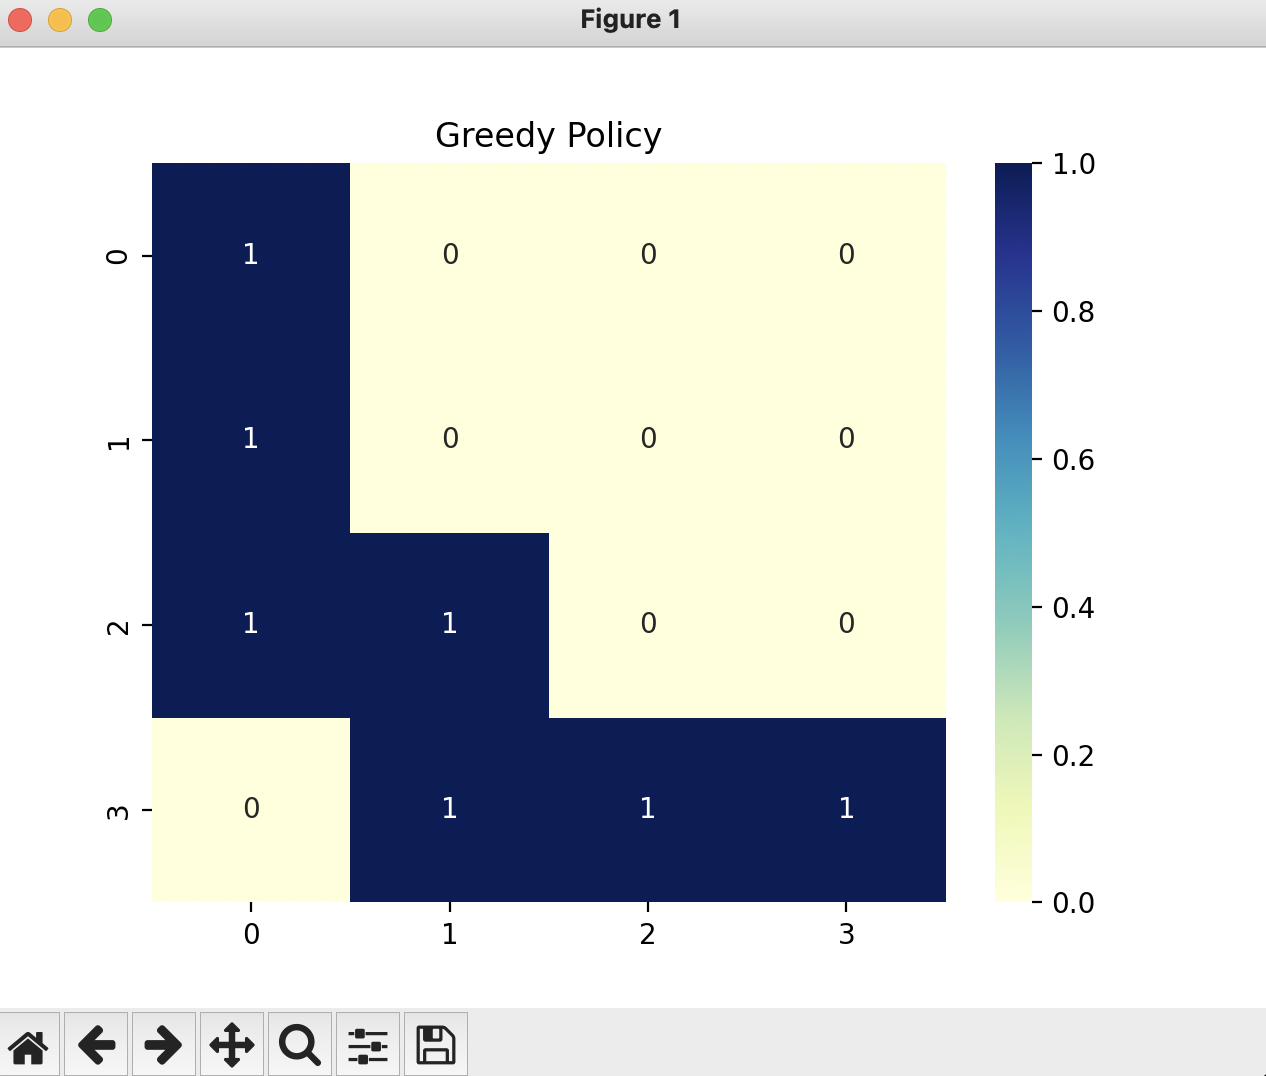
\includegraphics[width=0.85\textwidth]{images/greedypolicy.png}
    \caption{The corresponding greedy policy to the utilities}
    \label{fig:image2}
\end{figure}

\subsection*{Conclusion}

The implemented value iteration algorithm seems to find the optimal policy for the given MDP.

\end{document}